
\section{$n$-vector model}
\label{sec:nVector}

The $n$-vector model describes a classical system of $n$-dimensional classical spins $s_i$ of unit length interacting on a lattice. It is a generalization of the Ising model where each spin can have a continuous set of values. The Hamiltonian is then

\begin{equation}
    H = -J\sum_{\langle ij \rangle} s_i \cdot s_j
\end{equation}

where $J$ is the bond strength and $\langle ij \rangle$ refers to a nearest neighbour interaction.

\section{XY model}
\label{sec:XYModel}

A special case of the $n$-vector model is the XY model when $n = 2$. Here the spins are two dimensional rotors as $s_i = (\cos \theta_i, \  \sin \theta_i)$. This yields the Hamiltonian

\begin{equation}
    H = - J \sum_{\langle ij \rangle} \cos(\theta_i - \theta_j)
\end{equation}

The partition function is therefore

\begin{equation}
    Z = \prod_i \int \frac{\mathrm d \theta_i}{2 \pi} e^{-\beta H} = \prod_i \int \frac{\mathrm d \theta_i}{2 \pi} e^{K \sum_{\langle ij \rangle} \cos(\theta_i - \theta_j)}
\label{eq:xypart1}
\end{equation}

where $K = J \beta$.

\subsection{Loop expansion}
\label{subsec:XYLoopexp}

Since equation (\ref{eq:xypart1}) is invariant under the transformation $\theta_i - \theta_j \rightarrow \theta_i - \theta_j + 2 \pi n$, $n \in \mathbb{Z}$, it can be expanded using the identity

\begin{equation}
    e^{\alpha \cos \beta} = \sum_{\gamma = -\infty}^{\infty} I_\gamma ( \alpha ) e^{i \gamma \beta}
\end{equation}

where $I_\gamma(\alpha)$ is the modified Bessel function. Using that $e^{\sum_i x_i} = \prod_i e^{x_i}$

\begin{align}
    Z &= \prod_i \int \frac{\mathrm d \theta_i}{2 \pi} \sum_{J_{\langle ij \rangle} = -\infty}^{\infty} \prod_{b = \langle ij \rangle} I_{J_{\langle ij \rangle}} ( K ) e^{iK J_{\langle ij \rangle} (\theta_i - \theta_j)} \\
\label{eq:xypart2}
% 
    &=  \prod_i \sum_{J_b} \left ( \int \frac{\mathrm d \theta_i}{2 \pi} e^{i N_i (\theta_i - \theta_j)} \right ) \left ( \prod_b I_{J_b} \right ) 
\end{align}

Where in the last step, $\prod_{\langle ij \rangle} e^{iKJ_{\langle ij \rangle} (\theta_i - \theta_j)} = e^{iN_i (\theta_i - \theta_j)}$. $N_i$ is therefore the sum of $J$ for the nearest neighbours of site $i$. Noting that

\begin{equation}
    \int \frac{\mathrm d \theta_i}{2 \pi} e^{i N_i (\theta_i - \theta_j)} = C \delta_{N_i 0}
\end{equation}

leads to the conclusion that the sum of incoming and outgoing flux $J$ into a site $i$ must be zero, in other words, the configurations are divergence free. This in turn means that a configuration of the system must contain closed loops of flux $J$.

% NOTE: Explanation to the last sentence; take one site i and impose that it has to be divergence free (some flux out, same flux in). Then impose the same thing on its neighbour. The flux coming out of i must flow into the neighbour. Repeating this process over the whole lattice will give closed loops.

\subsection{Winding number}
\label{subsec:XYWindingNum}

In the ground state all the spins are aligned, while at higher energy states, the spins are pointed in random directions as can be seen in figure (\ref{fig:xygroundhigher}).

\begin{figure}[h!]
\centering
    \begin{subfigure}{.4\textwidth}
        \centering
        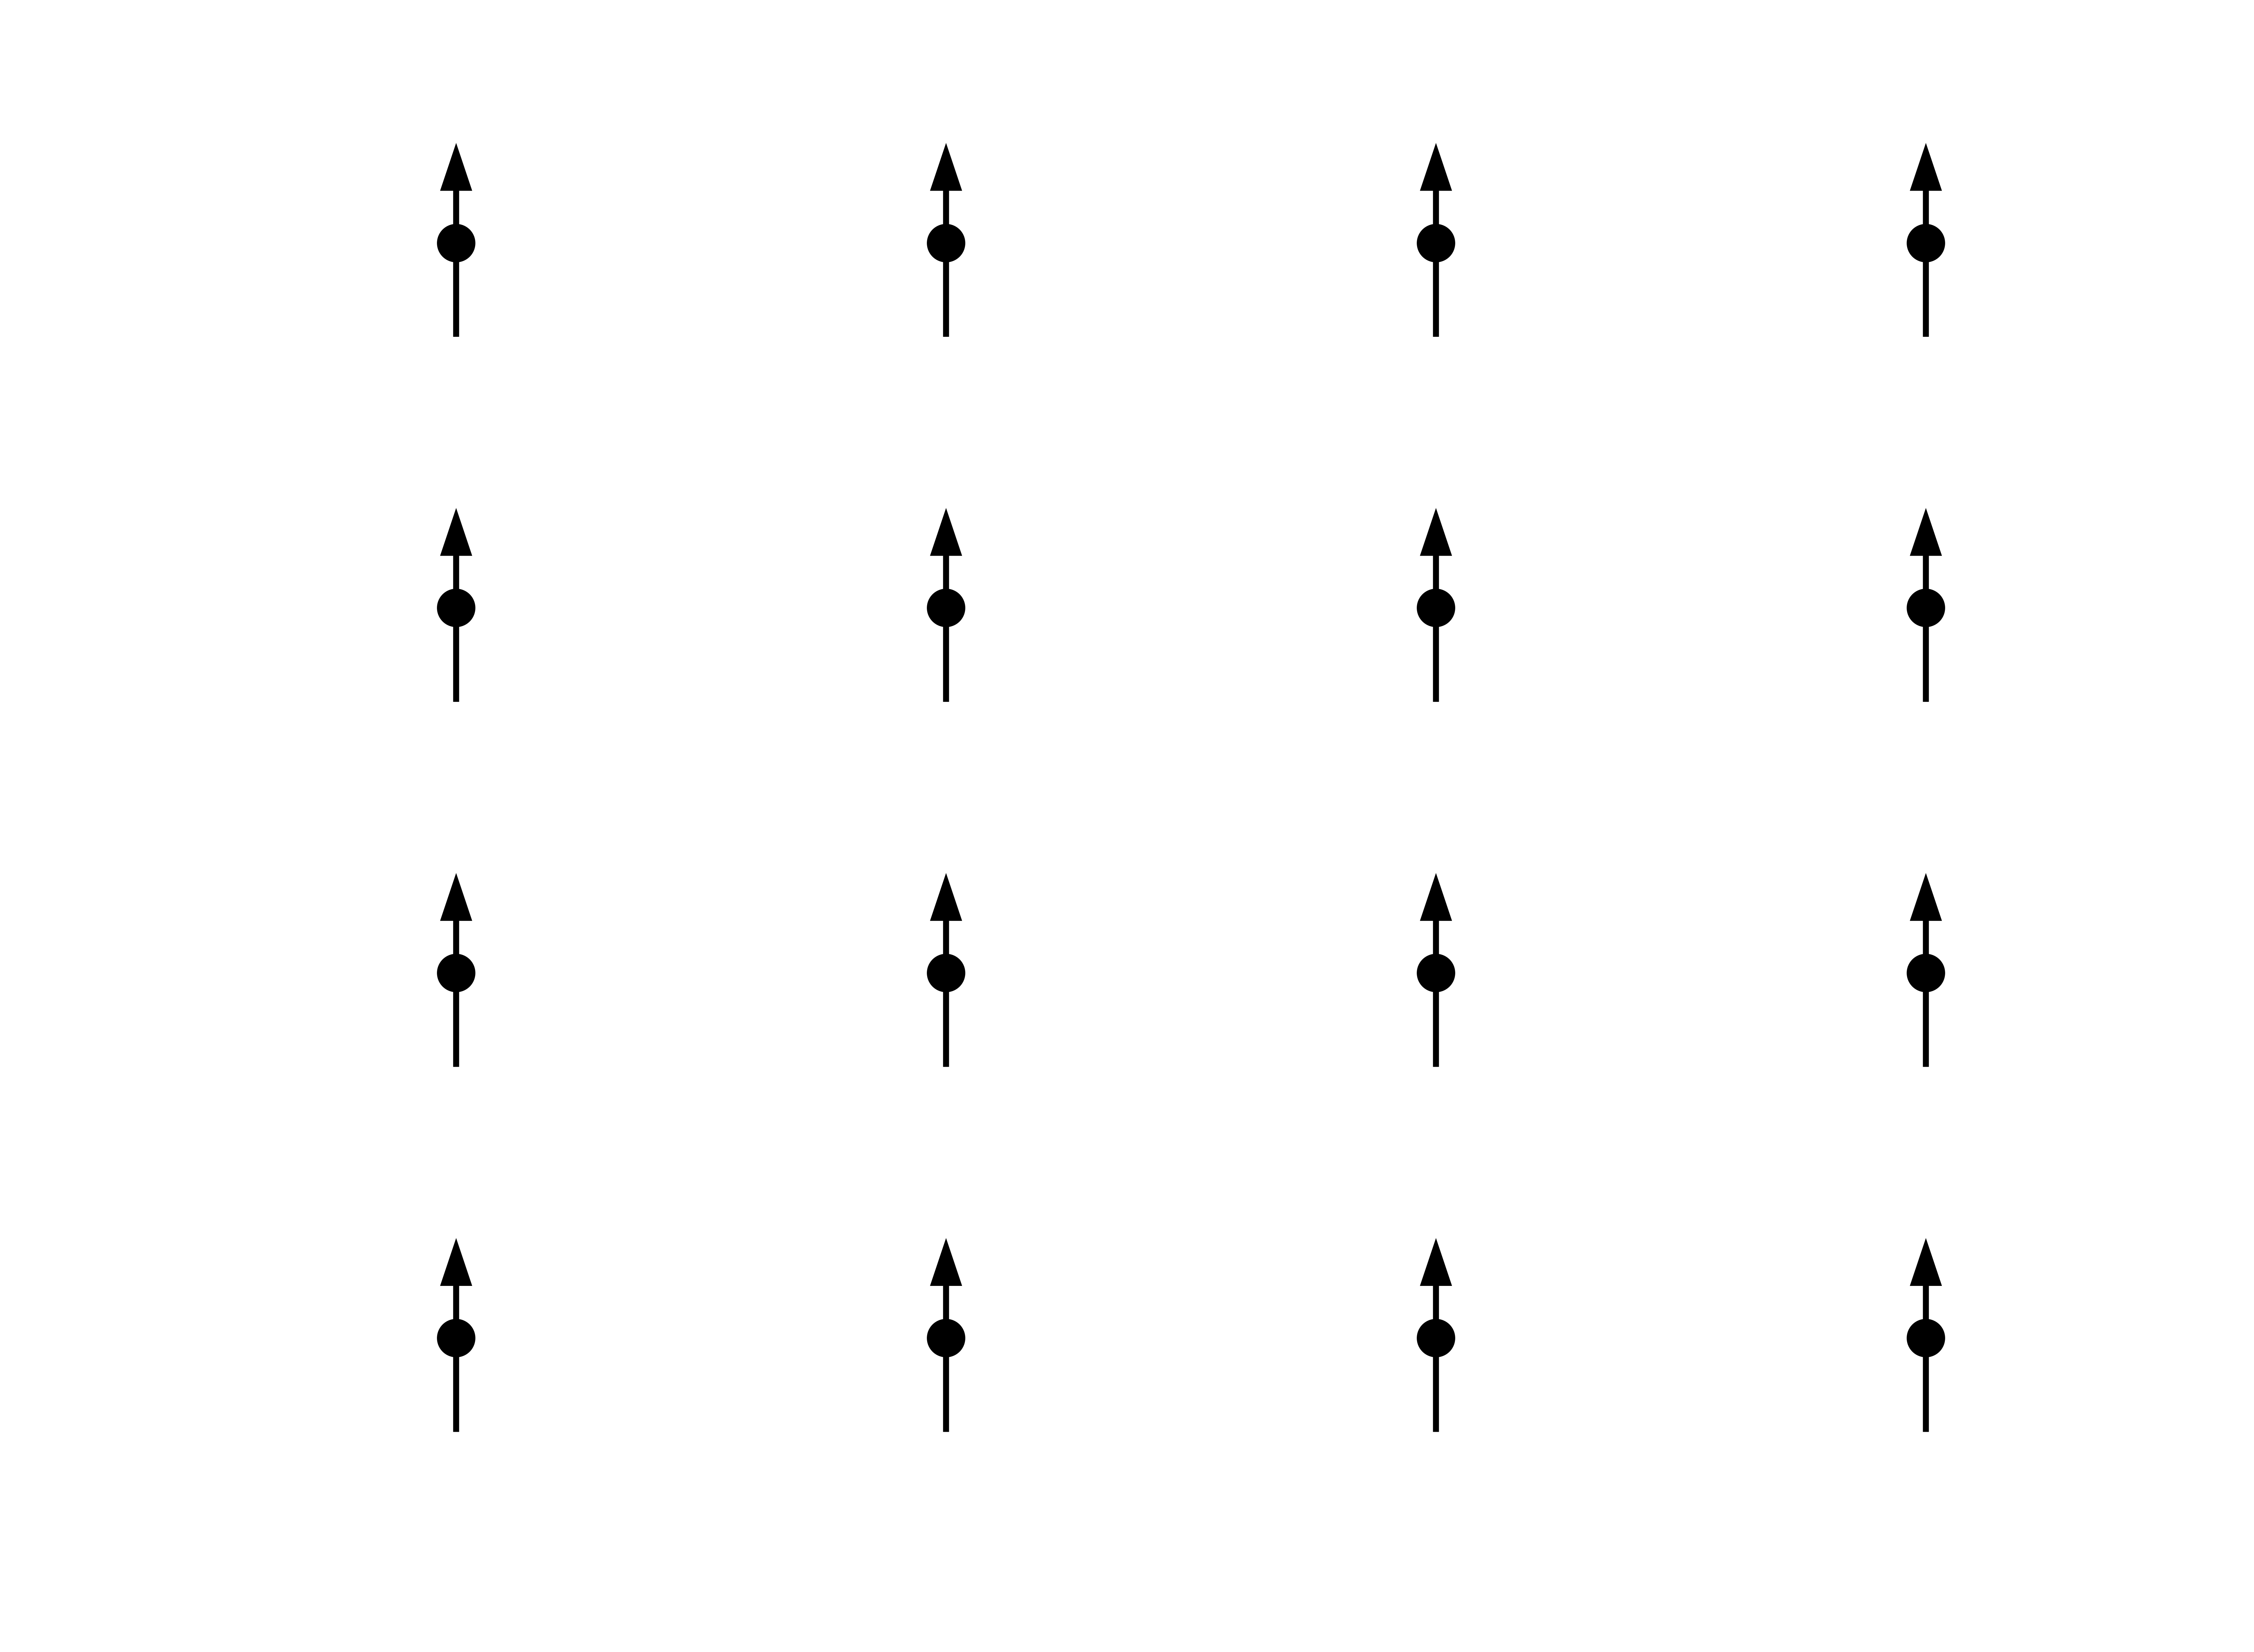
\includegraphics[width=\linewidth]{figures/noPhaseShift.png}
        \caption{Ground state}
        \label{fig:xyground}
    \end{subfigure}%
    \begin{subfigure}{.4\textwidth}
        \centering
        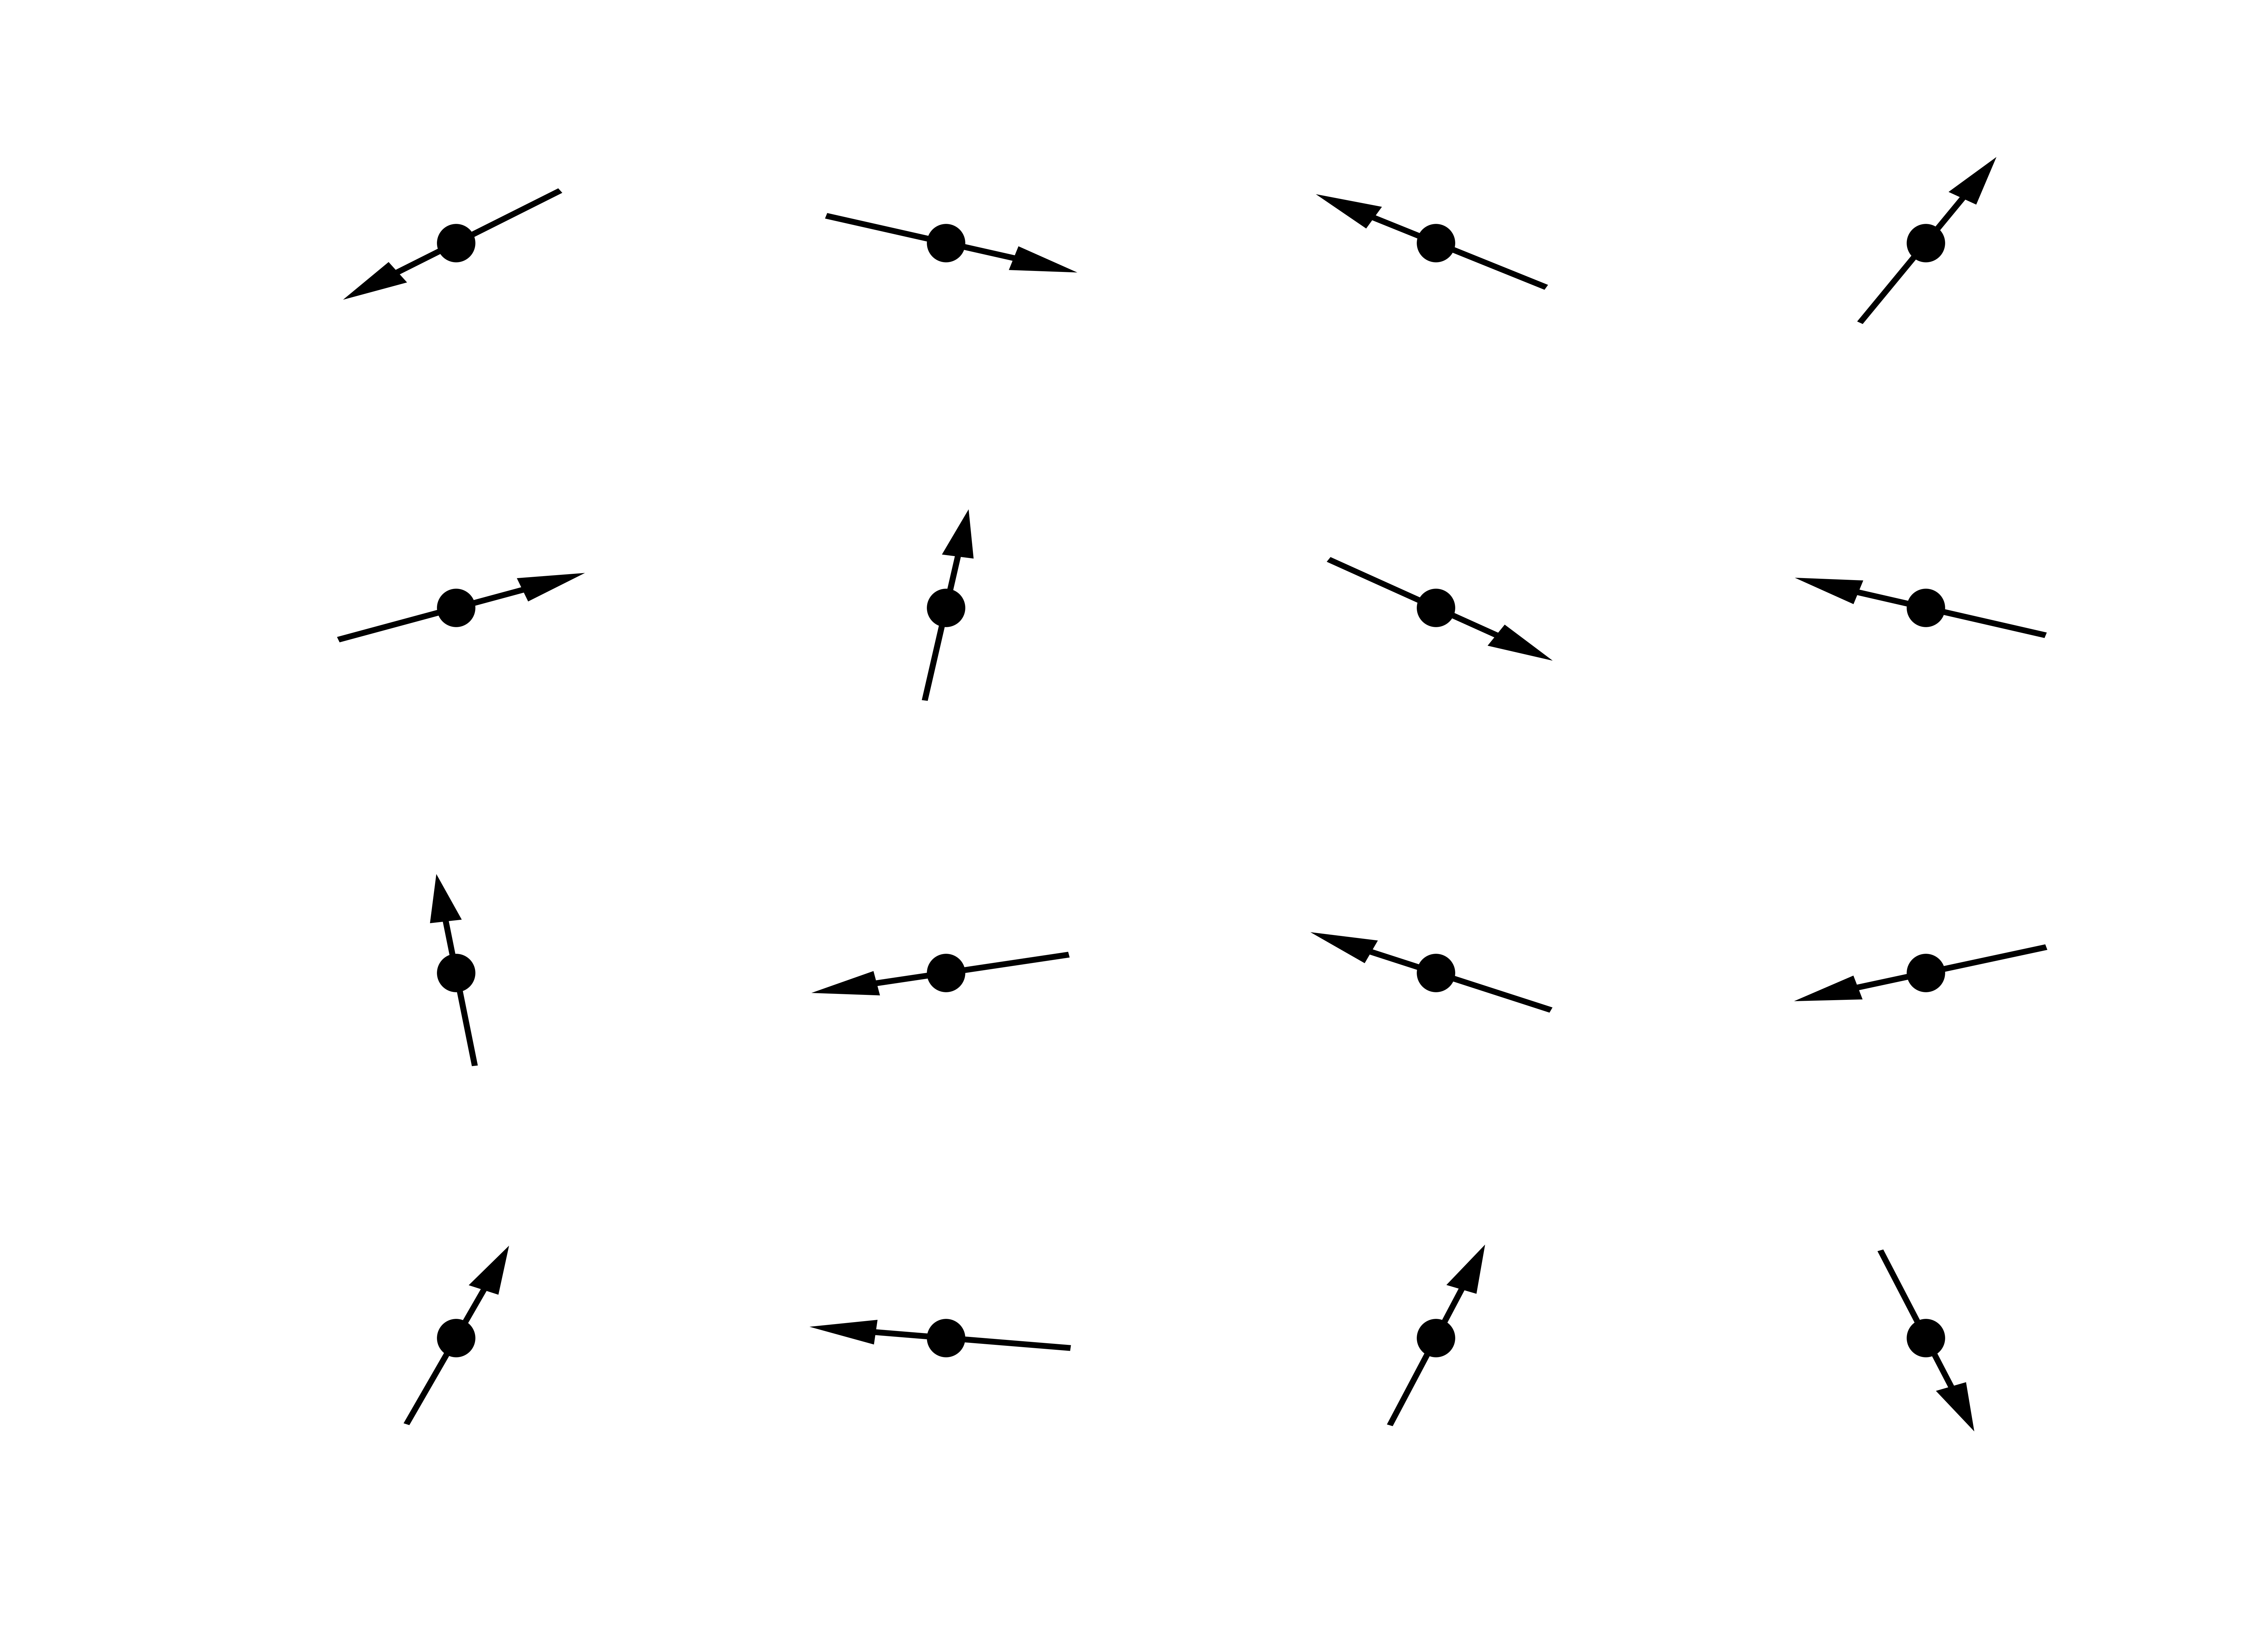
\includegraphics[width=\linewidth]{figures/randomAngle.png}
        \caption{Higher energy state}
        \label{fig:xyhigher}
    \end{subfigure}
    \caption{Energy states for XY model}
\label{fig:xygroundhigher}
\end{figure}

Therefore, making a constant phase shift $\Phi_\mu = \frac{A}{L}$ of $\theta_i - \theta_j$ in the $\mu$ direction would change the energy drastically for the ground state while, on a statistical average, not change the higher states energy at all (see figure (\ref{fig:xyphaseshift})).

\begin{figure}[h!]
\centering
    \begin{subfigure}{.4\textwidth}
        \centering
        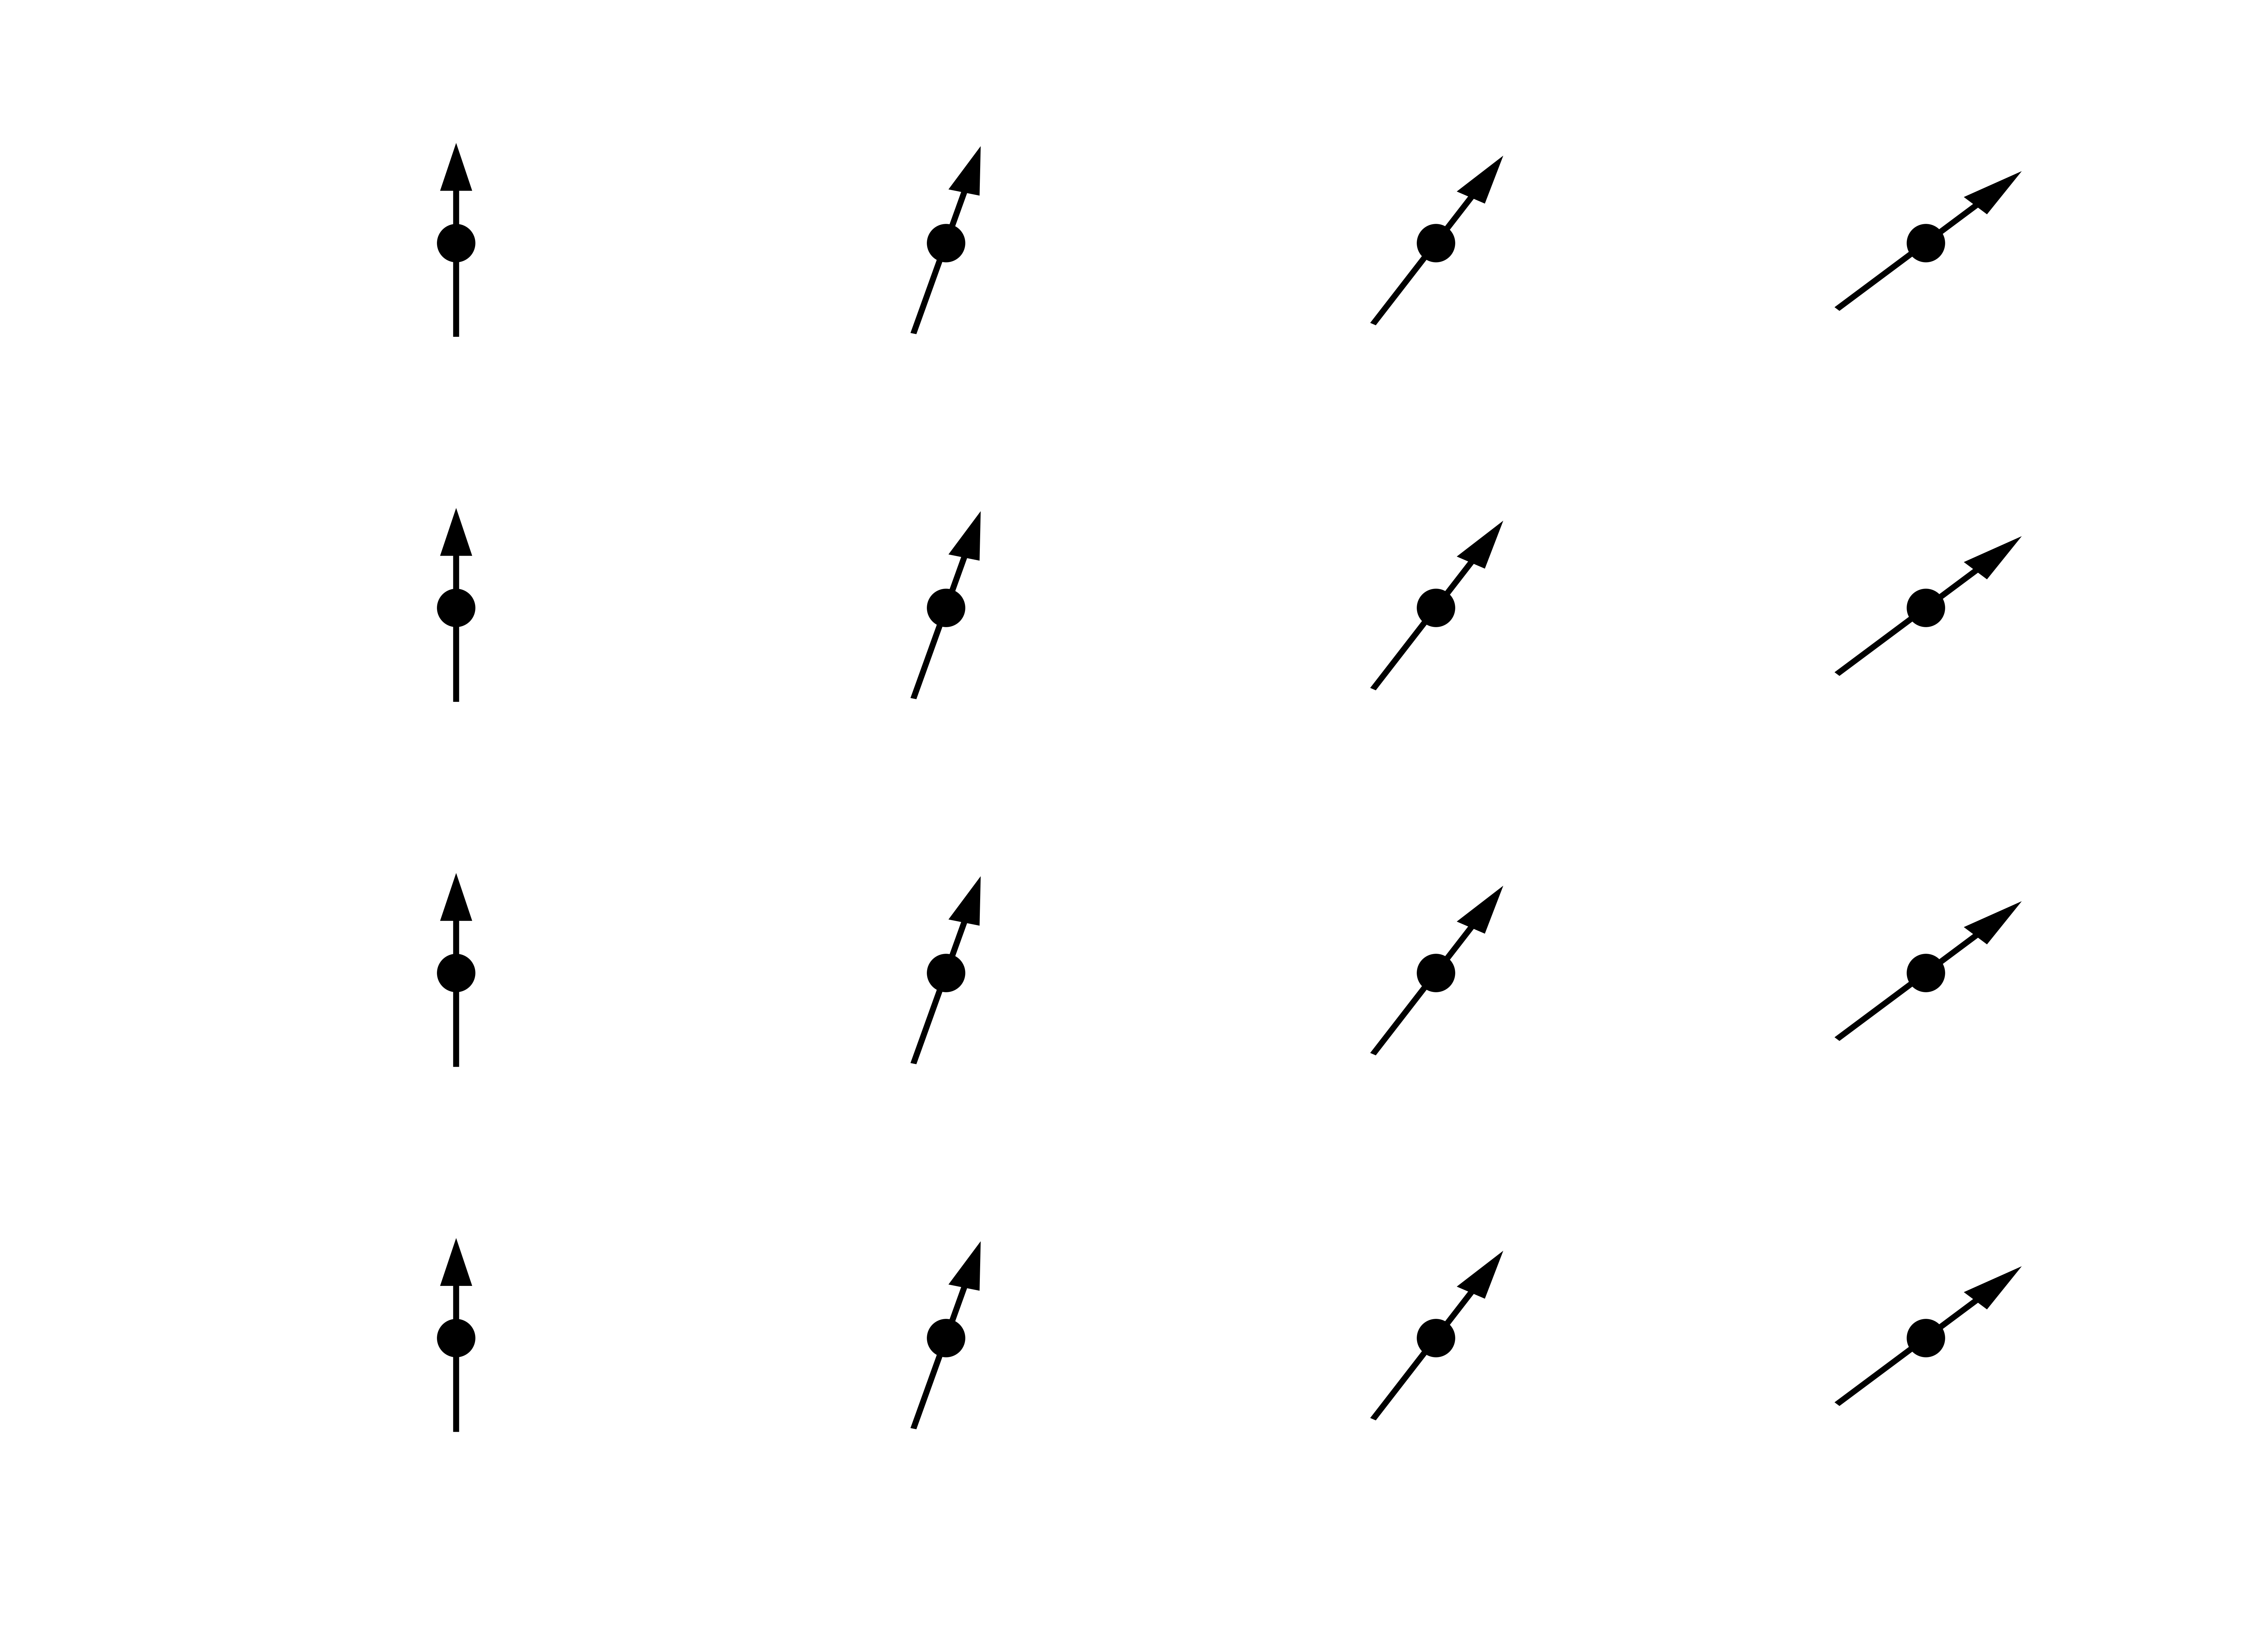
\includegraphics[width=\linewidth]{figures/phaseShiftXaxis.png}
        \caption{Ground state}
        \label{fig:xyground}
    \end{subfigure}%
    \begin{subfigure}{.4\textwidth}
        \centering
        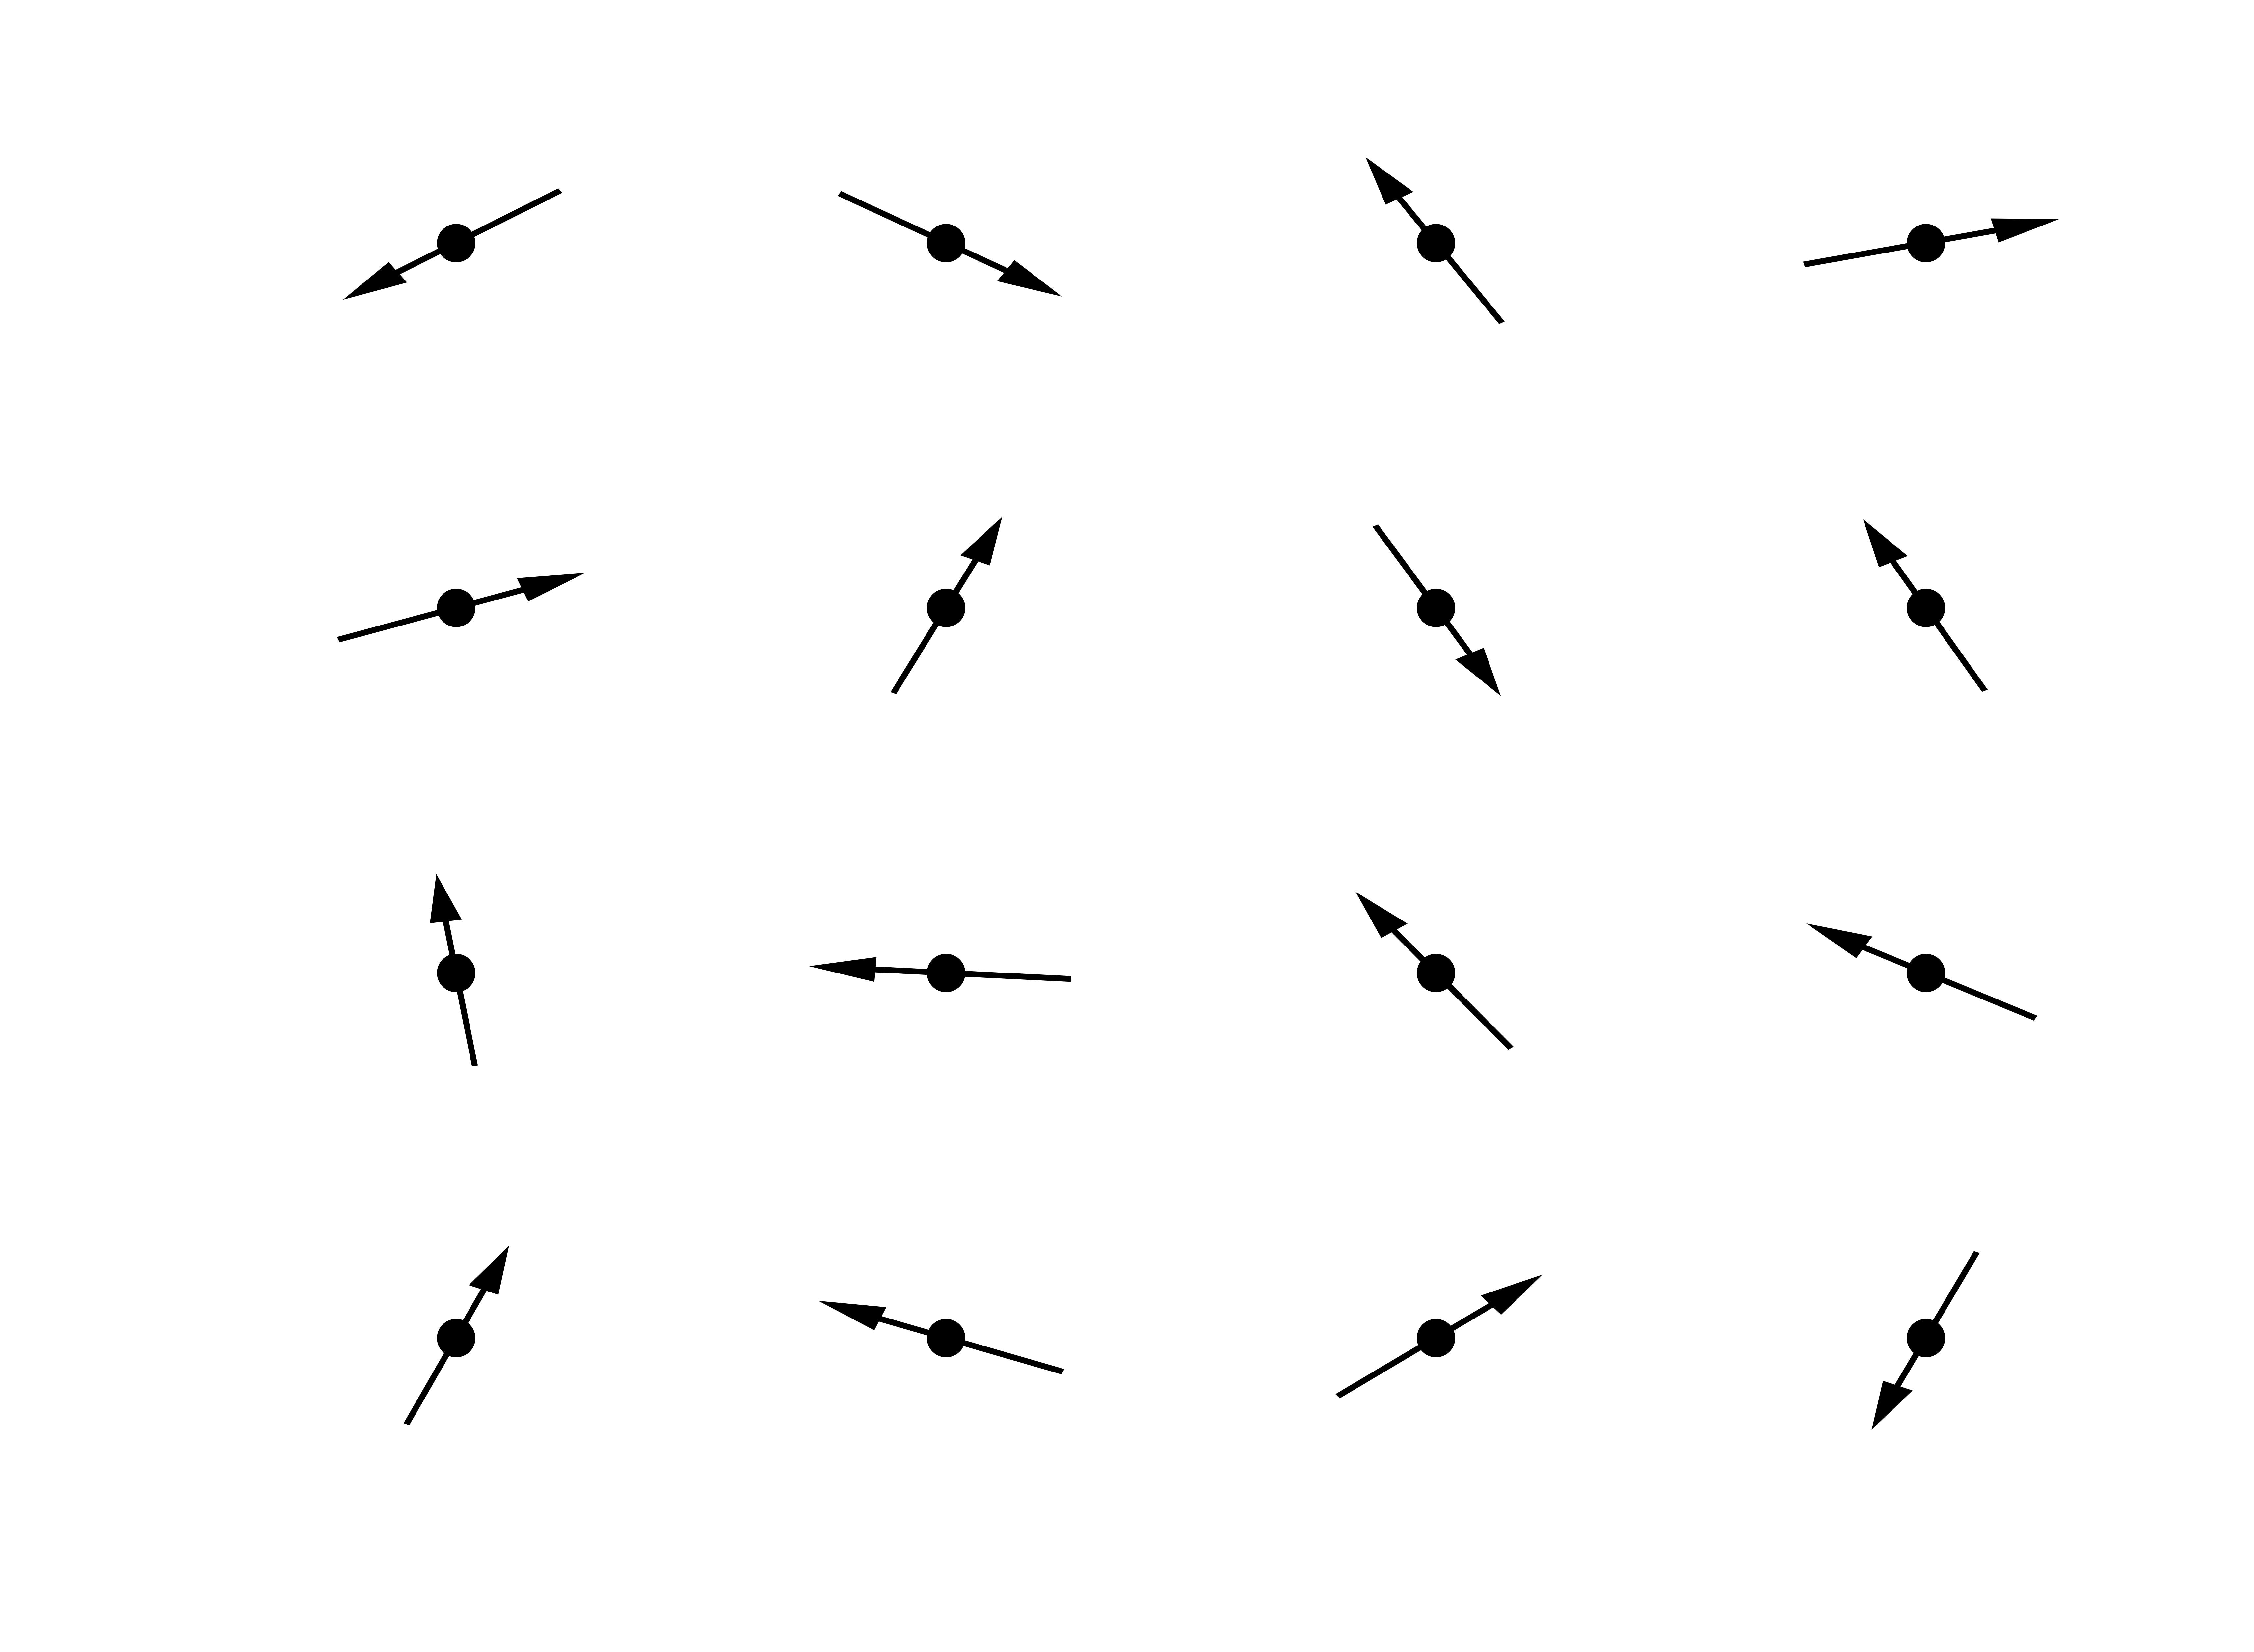
\includegraphics[width=\linewidth]{figures/randomPhaseShift.png}
        \caption{Higher energy state}
        \label{fig:xyhigher}
    \end{subfigure}
    \caption{A phase shift for $\mu = x$}
\label{fig:xyphaseshift}
\end{figure}

The free energy change $\Delta F$ for such a shift is

\begin{equation}
    \Delta F = L^d \cdot \frac{1}{2} \rho_s \left( \frac{A}{L} \right)^2 \Rightarrow \rho_s = \lim_{A \to 0} L^{2 - d}\frac{\partial^2 \Delta F}{\partial A^2}
\end{equation}

where $d$ is the dimension and $\rho_s$ is the superfluid density which is zero for a high energy state. The free energy is

\begin{equation}
F = - T \ln(Z) \Rightarrow F'' = T \left(\left(\frac{Z'}{Z}\right) - \left( \frac{Z''}{Z} \right)^2 \right)
\label{eq:xyfreeenergy}
\end{equation}

where $F' = \partial F / \partial A$. Examining $Z$ from (\ref{eq:xypart2}) with the added shift

\begin{align}
    Z &= \prod_i \int \frac{\mathrm d \theta_i}{2 \pi} \sum_{J_{\langle ij \rangle} = -\infty}^{\infty} \prod_{b = \langle ij \rangle} I_{J_{\langle ij \rangle}} ( K ) e^{iK J_{\langle ij \rangle} (\theta_i - \theta_j + \Phi_\mu)} \\
%
    & = \prod_i \sum_{J_b} \left ( \int \frac{\mathrm d \theta_i}{2 \pi} e^{i N_i (\theta_i - \theta_j)} \right ) \left ( \prod_b I_{J_b} \right ) \cdot e^{i K A \frac{1}{L} \sum_i J_{i, i+\mu}} \\
\label{eq:xypart3}
\end{align}

where in the last step

\begin{align}
    \prod_i \left (\prod_{\langle ij \rangle} e^{iK J_{\langle ij \rangle} \Phi_\mu} \right) &= \\
%
    \left\{ \text{$\Phi_\mu \neq 0$ only for neighbours in the $\mu$ direction} \right \} &= \\
%
    \prod_i \left ( e^{iK J_{i, i+\mu} \Phi_\mu} \right ) &= \\
%
    e^{iKA \frac{1}{L} \sum_i J_{i, i+\mu}}
\end{align}

Introduce the winding number in the $\mu$ direction as

\begin{equation}
    W_\mu = \frac{1}{L} \sum_i J_{i, i+\mu}
\label{eq:defwinding}
\end{equation}

Intuitively, this describes the net flux in the $\mu$-direction. Given a loop within the bounds of the lattice, the winding number is always zero. This is since an equal amount of flux in $+\mu$ as in $-\mu$ is needed to form a loop. However, this is not the case for a percolating cluster going, for example, from $-\mu$ to $+\mu$ connecting with periodic boundary conditions. For such a `winding' cluster, the winding number will be $+1$. An example can be seen in figure (\ref{fig:fluxpercolation}).

\begin{figure}[h!]
    \centering
        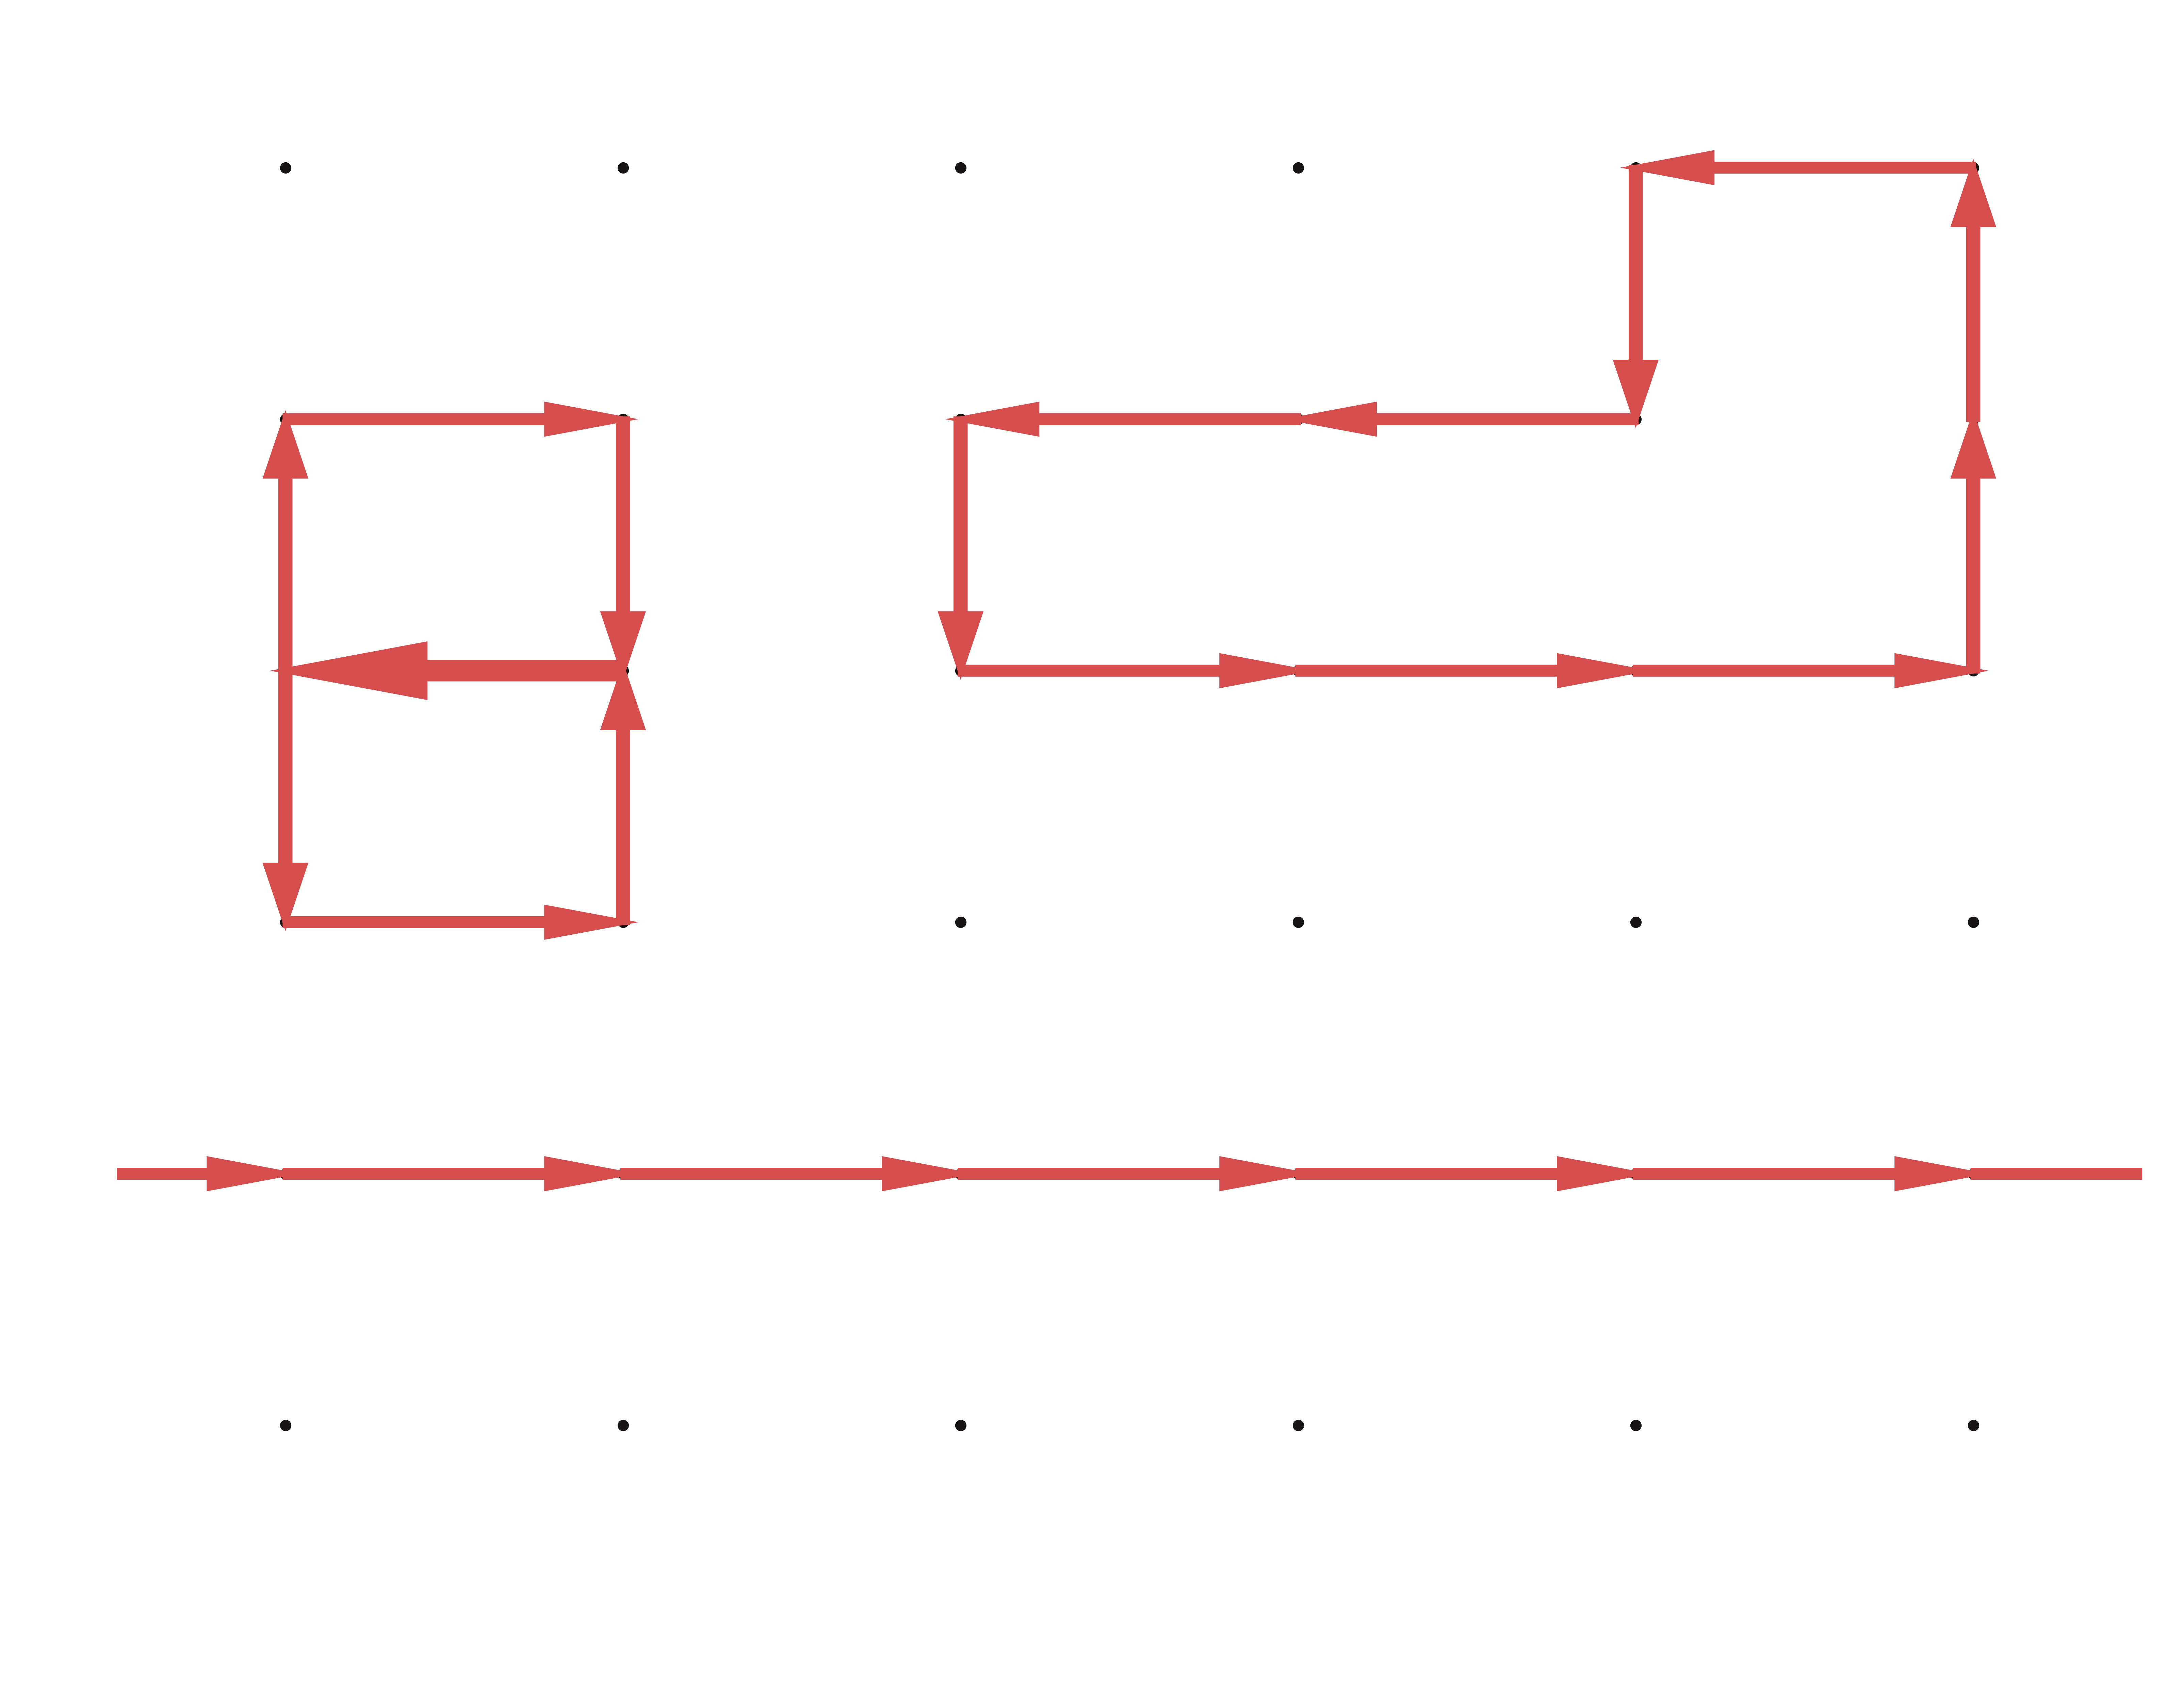
\includegraphics[width=0.6\textwidth]{figures/percolatingFlux.png}
    \caption{Three flux clusters on a square lattice. One percolating cluster with $W_x = +1$. The size of arrow corresponds to the number of flux quanta between two sites.}
    \label{fig:fluxpercolation}
\end{figure}

Using the definition (\ref{eq:defwinding}) for the winding number in the partition function in equation (\ref{eq:xypart3}) yields

\begin{align}
    Z &= \sum_{J_b} \left ( \prod_b I_{J_b} \right ) \prod_i \left ( \int \frac{\mathrm d \theta_i}{2 \pi} e^{i N_i (\theta_i - \theta_j)} \right ) \cdot e^{i K A W_\mu} \\
    &= \sum_{J_b, \ N_i = 0} Z_0 \cdot e^{i K A W_\mu} \\
    &= \sum_{W_\mu} Z_0 \cdot e^{i K A W_\mu}
\end{align}

Using this result in equation (\ref{eq:xyfreeenergy})

\begin{align}
    \frac{\partial^2 F}{\partial A^2} &= T \left ( \left ( \frac{\sum_{W_\mu} (i K W_\mu) Z_0 e^{iKAW_\mu}}{\sum_{W_\mu} Z_0 e^{iKAW_\mu}} \right )^2 - \frac{\sum_{W_\mu} (- K^2 W_\mu^2) Z_0 e^{iKAW_\mu}}{\sum_{W_\mu} Z_0 e^{iKAW_\mu}} \right ) \\
%
    &= T K^2 \left ( -\langle W_\mu \rangle^2 + \langle W_\mu^2 \rangle \right ) \\
%
    &= T K^2 \langle W_\mu^2 \rangle
\end{align}

Where $\langle W_\mu \rangle = 0$ since there is an equal chance of percolating from $-\mu$ to $\mu$ as the other way around.

The superfluid density can finally be determined as

\begin{equation}
    \rho_s = L^{2 - d} T K^2 \langle W_\mu^2 \rangle 
\end{equation}

